 \raggedright
\section{Autocorrelation implementation}
The Author's code starts here. How do we implement Autocorrelation using statsmodel library?
Firstly import acf function from statsmodel library insuring it is previously downloaded onto the computer \cite{statsmodel}. Code and print results seen on Figure \ref{a} explain how to import the library as well as calling the function with our dataset (variable `signal'). 

\begin{python}
from statsmodels.tsa.stattools import acf
#Autocorrelate the signal and plot
#signal is the variable with all the raw data
acorr = acf(signal, nlags=(len(signal)))
plt.plot(acorr)
\end{python}

\begin{figure}[ht]
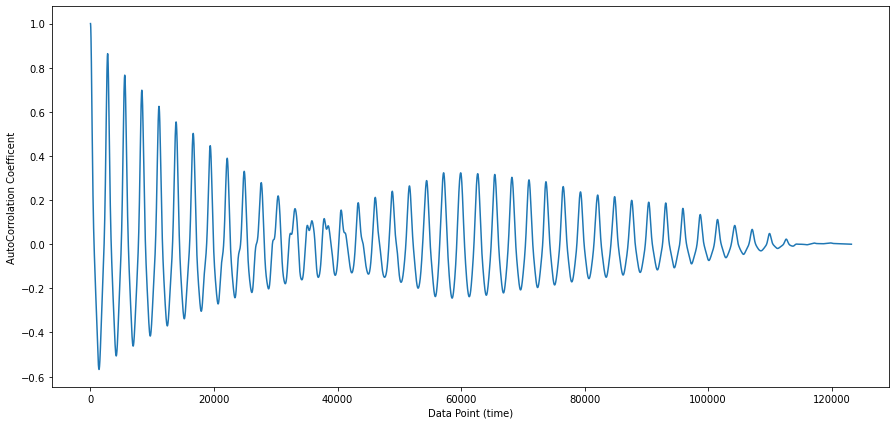
\includegraphics[scale=0.45]{images/autocorrolationCoefficent.png}
\caption{Output}
\label{a}
\end{figure}
The number of lags is equal to the total number of datapoints in plot \ref{a}.
Every peak is a point where the function found a correlation i.e pattern. This explains why at datapoint zero the coefficient of autocorrelation is 1 (100\%) as the script has not had enough time to shift itself by $n$ lags.
The next step is to extract the sections that have relatively high autocorrelation coefficient. This is done by recording all datapoints `peaks'.The process of peaks in the next step can create limitations we will talk about in section \ref{limitation}.


\begin{python}
peak_points = scipy.signal.find_peaks(acorr, height=0.1,prominence=0.2)
plt.ylabel('AutoCorrolation Coefficent')
plt.xlabel('time (datapoints)')
plt.plot(acorr)
plt.plot(peak_points[0],peak_points[1]['peak_heights'],'rx') 
#rx = crosses
\end{python}

\begin{figure}[ht]

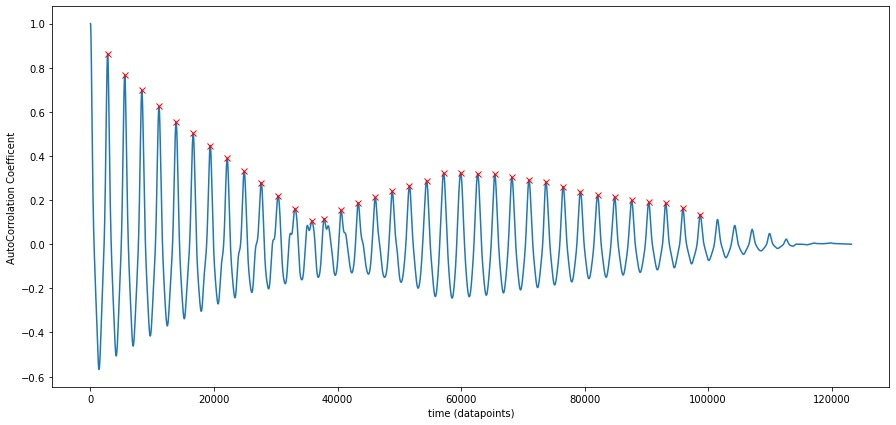
\includegraphics[scale=0.45]{autocorrolationCoefficentWithPeaks.jpg}
\caption{Output}
\label{autocorrolaiton with peaks}
\end{figure}

``peak\_points" array produces a list where in the 123,200 total datapoints the correlation is taking place. In other words, each value in ‘peaks’ array represents a pattern. The next step is to join 2 adjacent peaks to create a start and end of a cycle. This was done using python's built in zip() function. The zip() function returns a zip object, which is an iterator of tuples where the first item in each passed iterator is paired together, and then the second item in each passed iterator are paired together etc.\cite{defZip}. Code in \ref{Paired List} sampled from \cite{paiedList}.

\begin{figure}[ht]
\centering

\begin{python}
"""Creating the timestamps from the peaks""" 
#using zip() + list slicing 
#to perform pair iteration in list
timestamps = list(zip(peaks, peaks[1:] + peaks[:1]))
print("Total cycles",len(timestamps))
# printing result
print ("The pair list is : " + str(timestamps))
\end{python}

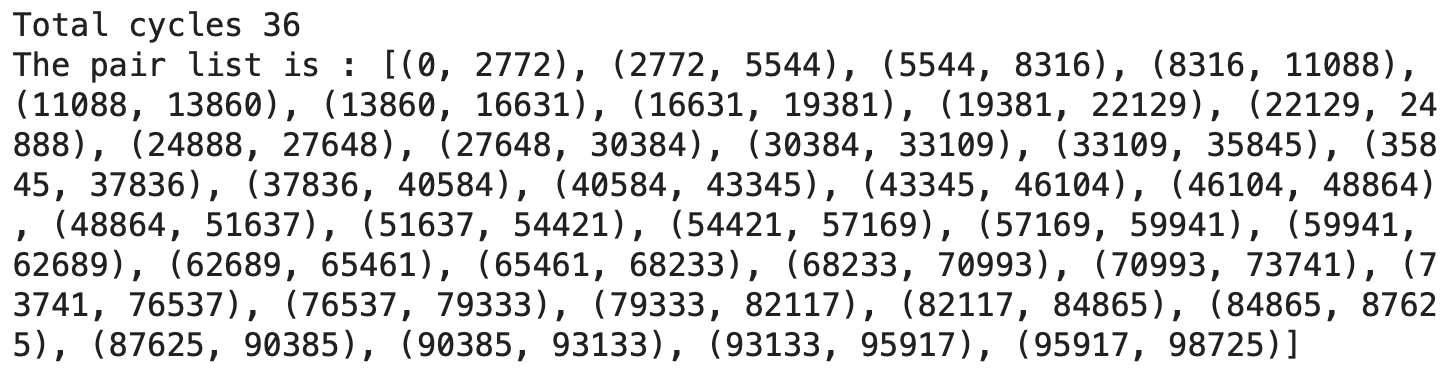
\includegraphics[scale=0.5]{images/arrayPeaks.png}
\caption{Paired List}
\label{Paired List}
\end{figure}

As you can see in figure \ref{Paired List}, we have converted the 37 
`crosses' into 36 cycles with start and end timestamps. List `timestamps' plotted shown on fig \ref{OverlayedCycles}.


\section{Filtering} \label{filtering}
Back to the initial objective, ``Identify a Representative cycle within the larger data set". Next step is deciding which cycle we should pick from the 36 cycles identified. 
\begin{figure}[ht]

\begin{python}
for cycle in cycles_plot:
    plt.plot(cycle)
\end{python}

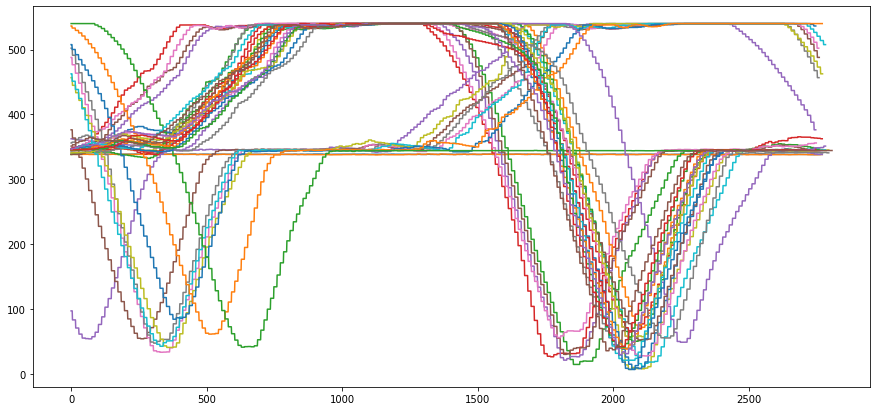
\includegraphics[scale=0.45]{images/cyclesOverlayed.png}
\caption{OverlayedCycles}
\label{OverlayedCycles}
\end{figure}


\subsection{Initial observations:}
\begin{itemize}

    \item Not all the cycles align.
    
    \item All the cycles seem to follow the large dip at time 2000.
    
    \item This dataset seems to have a cap at magnitude of roughly
    500.
    \item Autocorrolation did a good job with this set of data.
    
    \item Some cycles seem longer than others.
    
    \item  The cycles don't all start at the same magnitude 
    
    \item Visually the cycles are very similar.
    
\end{itemize}

\subsection{Maximum peak}
Approach A: filter with maximum peak, lowest trough, largest range 

This approach would give the most extreme cycles. While it is a "...Representative cycle...". It isn't the closest to the "average"

\begin{python}
listforMax=[]

for i in cycles_plot:
    listforMax.append(max(i))    
    
maxIndex = listforMax.index(max(listforMax))

\end{python}

The `for loop' finds the maximum value for each cycle in cycles\_plot then adds it to `listforMax'. Once the loop finishes, it has 36 values, one maximum value for each cycle. If we want to select the cycle with the largest value, variable `maxIndex', holds the index value of this cycle. In our case it is index nº 4.

\subsection{Lowest trough}

\begin{python}
listforMin=[]

for i in cycles_plot:
    listforMin.append(min(i))
    
minIndex = listforMin.index(min(listforMin))

\end{python}

The `for loop' finds the minimum value for each cycle in `cycles\_plot' and then adds it to `listforMin'. Once the loop finishes it has 36 values, one minimum value for each cycle. If we want to select the cycle with the lowest value, variable `minIndex' holds the index value of this cycle. In our case it is index nº 30.

\subsection{Average}
After using the mathematical average approach to find the average peak of all the magnitudes of each cycle, we must find the mean of the 36 values. For the purposes of comprehension, assume it gives us a value of 340.2, and then use Python built in method index() to find the cycle number. Unfortunately the mean or average value calculated might not exist in the actual data, giving the script an error. Instead we have to alter this approach and find the closest real value to the theoretical mean. This is an approach: 

\begin{python}
meanList=[]
for i in cycles_plot:

    meanList.append(np.sum(i)/len(i))
\end{python}

Here we have created a list with 36 values, the overall mean magnitude per cycle, giving the length of this list equal to the total number of cycles found from the Autocorrolation function. 
Next is finding the index and closest real value. 
\begin{python}
closest_real_value = min(meanList, key=lambda x:abs(x-np.average(meanList)))
closest_to_av_index = meanList.index(closest_real_value)

print(closest_to_av_index)
\end{python}

Using Python's built in min function, it finds the minimum distance from the ´meanList' to the real value ``np.average(meanList)". \cite{realValue}

The `meanList.Index()' function finds the index of our  ´closest\_real\_value' Giving an output of cycle nº 13.

\subsection{Filtering limitations}
Average, minimum and maximum work in the authors case but everyone's use case is different. Exploring other options like Standard deviations, most common cycle, 25 quarterly could be explored. 
\section{Autocorrelation limitation}\label{limitation}

When the signal data has a greater Randomness the magnitude of the Autocorrelation coefficient is reduced drastically. 

The lower the amount of cycles found, the higher the probability that the cycle selected is not ``...Representative...". 

\begin{figure}[ht]
\centering
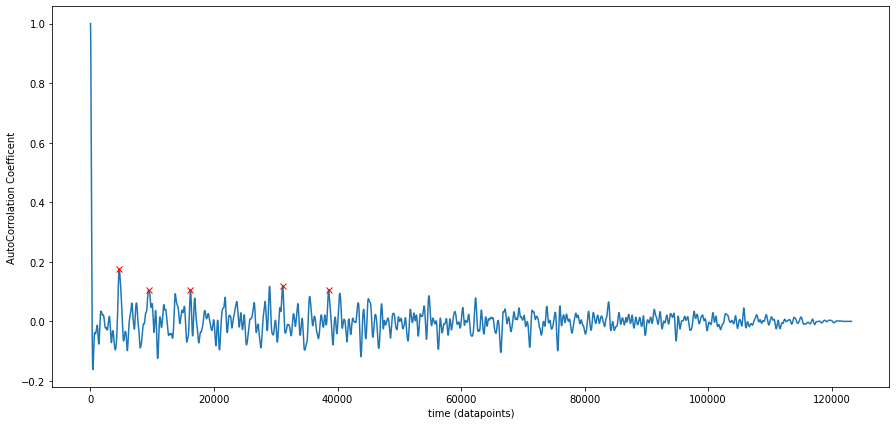
\includegraphics[scale=0.40]{images/autocorrolationBadCoefficentWithPeaks.png}
\caption{Limit Testing A}
\label{LimitA}
\end{figure}

Stress testing 'acf' function with dataset B, the displacement steering cylinder dataset has a higher randomness compared to the dataset A used in the rest of the report. This translates to a decrease in total cycles found. The amount of cycles identified went from 36 to 5, 86\% decrease. 
This can be justified as the steering cylinder has a lot of feedback from the machine's steer over rocks and uneven terrain unlike the lift or tilt cylinder.

\begin{figure}[ht]
\centering
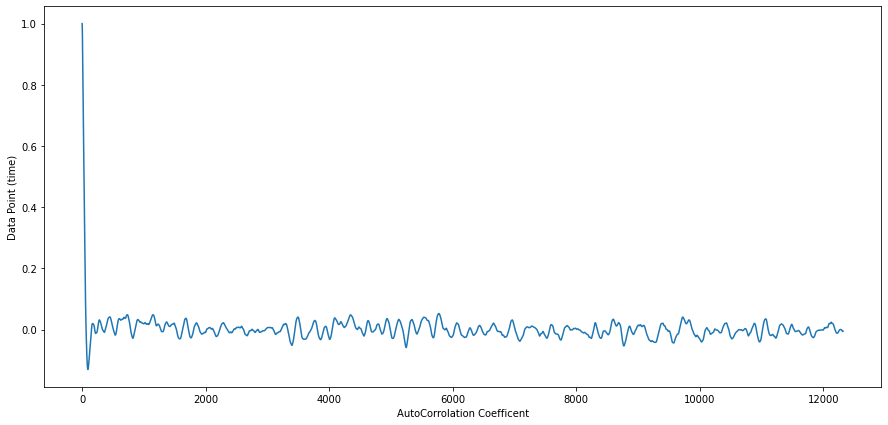
\includegraphics[scale=0.40]{images/limitTestB.png}
\caption{Limit Testing B }
\label{LimitB}
\end{figure}
The heaviest stress testing was with dataset C, ref \ref{LimitB}.This data came from a strain gauge force dataset attached to a CAT machine. Here the function failed to correlate a single Dataset. Factors for this result could be 500hz sensor data causing too much noise. Forces by nature are going to be harder to correlate compared to displacement. 
